\chapter{Physically Based Rendering}

In order to generate photorealistic images, renderers must find accurate solutions to the \textit{rendering equation}. This chapter explains the meaning and intuition behind the equation, and describes how it can be solved by the path-tracing algorithm.

\section{The Rendering Equation}

The rendering equation describes the ``strength'' of light at each point in space and in each direction. To formalize the notion of strength, this section begins by introducing a few concepts from the study of radiometry.

\subsection{Radiometry}

In radiometry, there is a hierarchy of quantities that measures the strength of light in different contexts. The first quantity is \textit{radiant flux}, which measures the total energy that travels through a region of space per unit time in the form of electromagnetic radiation. Radiant flux is often denoted by $\Phi$, and its unit of measure is Watts($W$). 

In almost all regions in any scene, the radiant flux is not uniformly distributed, and thus one important quantity is the density of radiant flux with respect to area. This quantity is named \textit{irradiance}, which is denoted by $E$, and measured in power per unit area ($W\cdot m^{-2}$). Intuitively, irradiance measures the amount of light received by a single point in space. For this reason, for a region of space $S$, integrating the irradiance of each point in $S$ gives the total flux through $S$:
\begin{align}
    \Phi(S) = \int_S E(p) dp 
    \label{irradiance integral}
\end{align}

For any point $p$, the irradiance $E(p)$ is not uniform across all directions, and thus it is also important to consider the density of irradiance in each direction $\omega$. This quantity, $L(p,\omega)$, is called \textit{radiance}, and its unit of measure for radiance is power per unit area per unit solid angle ($\text{W}\cdot\text{m}^{-2}\cdot \text{sr}^{-1}$). Radiance is an especially important quantity, because it is a measure of the strength of a single ray of light, identified by its direction $\omega$ and a point $p$ which it passes through. Consequently, radiance is the physical quantity that ray-tracing algorithms constantly operates in. 


In rendering, radiance often appears in the form $L_o(p,\omega)$ or $L_i(p,\omega)$, which mean radiance going out from the point $p$ or entering into it, respectively. More precisely, $L_o(p,\omega)$ represents the radiance that travels from $p$ and outwards in the direction $\omega$, and $L_i(p,\omega)$ represents the incoming radiance that travels towards to $p$ in the direction $-\omega$. The convention $L_i(p,\omega)$ might appear slightly counter-intuitive, since $\omega$ points in the opposite direction as the propagation of energy. However, the convenience of this notation will become apparent when the ray-tracing algorithm is formulated. 



\begin{figure}[H]
\centering
\tikzset{every picture/.style={line width=0.75pt}} %set default line width to 0.75pt        
\begin{tikzpicture}[x=0.75pt,y=0.75pt,yscale=-1,xscale=1]
%uncomment if require: \path (0,300); %set diagram left start at 0, and has height of 300

%Straight Lines [id:da6428603089338014] 
\draw    (70,220) -- (251,220) ;
\draw [shift={(160.5,220)}, rotate = 0] [color={rgb, 255:red, 0; green, 0; blue, 0 }  ][fill={rgb, 255:red, 0; green, 0; blue, 0 }  ][line width=0.75]      (0, 0) circle [x radius= 3.35, y radius= 3.35]   ;
%Straight Lines [id:da0998330538982608] 
\draw    (160.5,220) -- (218.58,162.41) ;
\draw [shift={(220,161)}, rotate = 495.24] [color={rgb, 255:red, 0; green, 0; blue, 0 }  ][line width=0.75]    (10.93,-3.29) .. controls (6.95,-1.4) and (3.31,-0.3) .. (0,0) .. controls (3.31,0.3) and (6.95,1.4) .. (10.93,3.29)   ;
%Straight Lines [id:da7334390340946089] 
\draw    (325,221) -- (506,221) ;
\draw [shift={(415.5,221)}, rotate = 0] [color={rgb, 255:red, 0; green, 0; blue, 0 }  ][fill={rgb, 255:red, 0; green, 0; blue, 0 }  ][line width=0.75]      (0, 0) circle [x radius= 3.35, y radius= 3.35]   ;
%Straight Lines [id:da024849495612862427] 
\draw    (480,160) -- (416.95,219.63) ;
\draw [shift={(415.5,221)}, rotate = 316.6] [color={rgb, 255:red, 0; green, 0; blue, 0 }  ][line width=0.75]    (10.93,-3.29) .. controls (6.95,-1.4) and (3.31,-0.3) .. (0,0) .. controls (3.31,0.3) and (6.95,1.4) .. (10.93,3.29)   ;
%Image [id:dp8436986937138125] 
\draw (161,245) node  {
\includegraphics[width=27pt,height=30pt]{lightbulb.png}};
%Image [id:dp5859653893638117] 
\draw (498,154) node  {
\includegraphics[width=27pt,height=30pt]{lightbulb.png}};

% Text Node
\draw (181,232) node [anchor=north west][inner sep=0.75pt]   [align=left] {$\displaystyle p$};
% Text Node
\draw (224,143) node [anchor=north west][inner sep=0.75pt]   [align=left] {$\displaystyle q$};
% Text Node
\draw (436,233) node [anchor=north west][inner sep=0.75pt]   [align=left] {$\displaystyle p$};
% Text Node
\draw (519,141) node [anchor=north west][inner sep=0.75pt]   [align=left] {$\displaystyle q$};


\end{tikzpicture}

\caption{Example: consider two points $p$, $q$, and $\omega=\frac{q-p}{|q-p|}$. On the left, the radiance sent from $p$ to $q$ is $L_o(p,\omega)$. On the right, the radiance received by $p$ from $q$ is $L_i(p,\omega)$.}
\end{figure}
Similar to equation \ref{irradiance integral}, which expresses flux as an integral of irradiance, it's also possible to obtain the incoming irradiance $E(p)$ by an integral across the incoming radiance from each direction. More precisely, the following relationship holds:
\begin{align}
    E(p) = \int_\Omega L_i(p,\omega_i)\cos\theta_id\omega_i
    \label{radiance integral}
\end{align}
Here, the support $\Omega$ is often a sphere or hemisphere of possible incoming direction, and the angle $\theta_i$ represents the angle between $\omega_i$ and the surface normal. The cosine term accounts for the fact that for incoming rays that are not perfectly perpendicular to the surface, the differential area illuminated by the ray is multiplied by a factor $\frac{1}{\cos\theta_i}$, and thus the contribution per unit area should be multiplied by $\cos\theta_i$. 
\begin{figure}[H]
    \centering
  



    \tikzset{every picture/.style={line width=0.75pt}} %set default line width to 0.75pt        

    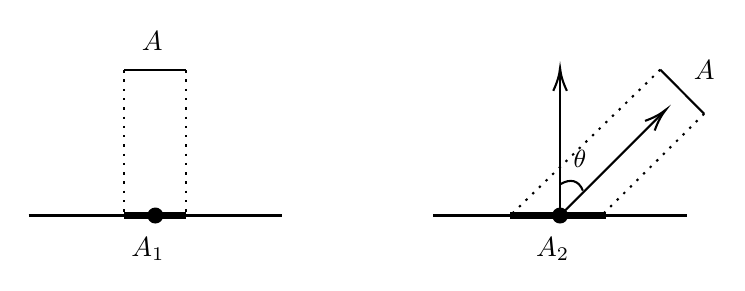
\begin{tikzpicture}[x=0.75pt,y=0.75pt,yscale=-1,xscale=1]
    %uncomment if require: \path (0,300); %set diagram left start at 0, and has height of 300
    
    %Straight Lines [id:da170514078900192] 
    \draw    (54,230) -- (176,230) ;
    \draw [shift={(115,230)}, rotate = 0] [color={rgb, 255:red, 0; green, 0; blue, 0 }  ][fill={rgb, 255:red, 0; green, 0; blue, 0 }  ][line width=0.75]      (0, 0) circle [x radius= 3.35, y radius= 3.35]   ;
    %Straight Lines [id:da016015541896946983] 
    \draw    (100,160) -- (130,160) ;
    %Straight Lines [id:da2875279917672757] 
    \draw  [dash pattern={on 0.84pt off 2.51pt}]  (100,160) -- (100,230) ;
    %Straight Lines [id:da4948721440011248] 
    \draw  [dash pattern={on 0.84pt off 2.51pt}]  (130,160) -- (130,230) ;
    %Straight Lines [id:da6791345652096885] 
    \draw [line width=2.25]    (100,230) -- (130,230) ;
    %Straight Lines [id:da17937256958328818] 
    \draw    (249,230) -- (371,230) ;
    \draw [shift={(310,230)}, rotate = 0] [color={rgb, 255:red, 0; green, 0; blue, 0 }  ][fill={rgb, 255:red, 0; green, 0; blue, 0 }  ][line width=0.75]      (0, 0) circle [x radius= 3.35, y radius= 3.35]   ;
    %Straight Lines [id:da5726229973180355] 
    \draw    (358.31,159.71) -- (379.42,181.02) ;
    %Straight Lines [id:da01972159484297009] 
    \draw  [dash pattern={on 0.84pt off 2.51pt}]  (358.31,159.71) -- (286,230) ;
    %Straight Lines [id:da8044979993297667] 
    \draw  [dash pattern={on 0.84pt off 2.51pt}]  (379.42,181.02) -- (329.69,230.29) ;
    %Straight Lines [id:da7389754977606782] 
    \draw [line width=2.25]    (286,230) -- (332,230) ;
    %Straight Lines [id:da7593939440598445] 
    \draw    (310,230) -- (310,161) ;
    \draw [shift={(310,159)}, rotate = 450] [color={rgb, 255:red, 0; green, 0; blue, 0 }  ][line width=0.75]    (10.93,-3.29) .. controls (6.95,-1.4) and (3.31,-0.3) .. (0,0) .. controls (3.31,0.3) and (6.95,1.4) .. (10.93,3.29)   ;
    %Straight Lines [id:da5048921054355329] 
    \draw    (310,230) -- (359.59,180.41) ;
    \draw [shift={(361,179)}, rotate = 495] [color={rgb, 255:red, 0; green, 0; blue, 0 }  ][line width=0.75]    (10.93,-3.29) .. controls (6.95,-1.4) and (3.31,-0.3) .. (0,0) .. controls (3.31,0.3) and (6.95,1.4) .. (10.93,3.29)   ;
    %Curve Lines [id:da665946044320908] 
    \draw    (310,215) .. controls (315,212) and (319,213) .. (321,218) ;
    
    % Text Node
    \draw (107,140) node [anchor=north west][inner sep=0.75pt]   [align=left] {$\displaystyle A$};
    % Text Node
    \draw (102,239) node [anchor=north west][inner sep=0.75pt]   [align=left] {$\displaystyle A_{1}$};
    % Text Node
    \draw (373,154) node [anchor=north west][inner sep=0.75pt]   [align=left] {$\displaystyle A$};
    % Text Node
    \draw (297,239) node [anchor=north west][inner sep=0.75pt]   [align=left] {$\displaystyle A_{2}$};
    % Text Node
    \draw (315,197) node [anchor=north west][inner sep=0.75pt]  [font=\small] [align=left] {$\displaystyle \theta $};
    
    
    \end{tikzpicture}
    

\caption{Example: on the right, the differential area $A_2$ illuminated by the ray is larger, because the ray is not perpendicular to the plane.}    
\end{figure}


\subsection{The BRDF}

In order to accurately model the incoming and outgoing radiances at each point, it is essential to take into account the fact that surfaces can reflect incoming light. That is, for any direction $\omega_i$, the incoming radiance $L_i(p,\omega_i)$ can contribute to the outgoing radiance $L_o(p,\omega_o)$ of another direction $\omega_o$. For each surface point, this relationship is captured by the bi-directional reflectance distribution function (BRDF), written as $f_r(p,\omega_o,\omega_i)$. Formally, the BRDF is defined as 
\begin{align}
    f_r(p,\omega_o,\omega_i) = \frac{dL_o(p,\omega_o)}{dE(p,\omega_i)}
    \label{BRDF def 1}
\end{align}
where $dE(p,\omega_i)$ represents the differential incoming irradiance in the direction $\omega_i$.

Using equation \ref{radiance integral}, it can be derived that 
\begin{align}
    dE(p,\omega_i) = L_i(p,\omega_i)\cos\theta_id\omega_i
\end{align}
which allows equation \ref{BRDF def 1} to be re-written as
\begin{align}
    f_r(p,\omega_o,\omega_i) = \frac{dL_o(p,\omega_o)}{L_i(p,\omega_i)\cos\theta_id\omega_i}
\end{align}
From this, it's straightforward to show that
\begin{align}
    L_o(p,\omega_o) = \int_\Omega f_r(p,\omega_o,\omega_i)L_i(p,\omega_i)\cos\theta_id\omega_i + C
    \label{reflection plus C}
\end{align}
for some $C$.

Equation \ref{reflection plus C} shows that, given the incident radiances and the BRDF, the portion of outgoing radiances caused by reflections can be computed. As a result, the BRDF of a surface completely decides how the surface reflects light, which is a crucial factor of its appearances when viewed by a camera. Different materials in the real world have drastically different BRDFs, and it's vital for a physically based renderer to accurately implement these functions, if photorealistic images are to be rendered. A family of BRDFs known for their physical accuracy are the Microfacet BRDFs, which are well implemented by this project. Unfortunately, due to the complexity of these models, details of these BRDFs could not be described here. 
\begin{figure}[H]
    \centering
    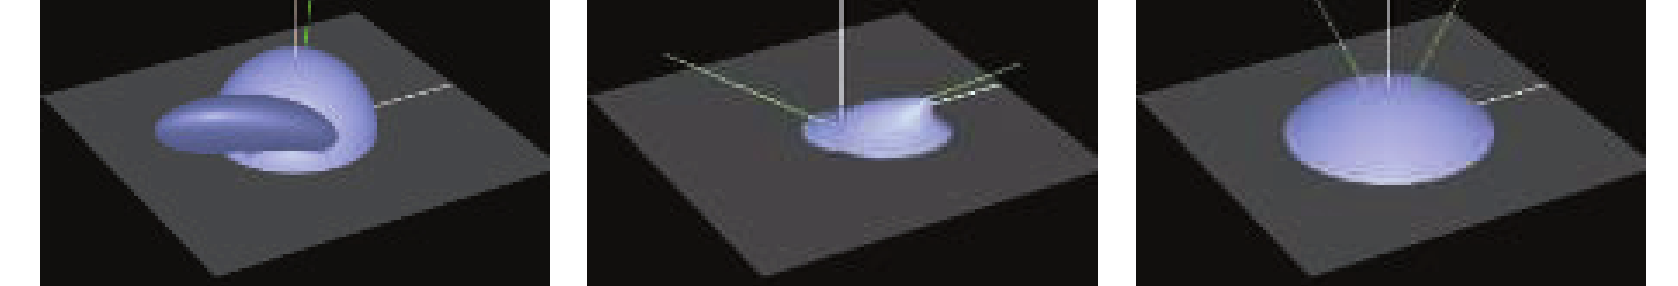
\includegraphics[scale = 0.6]{brdfs}
    \caption{Shapes of example BRDFs. Image credit\cite{akenine2019real}}
\end{figure}

In order to fully model $L_o(p,\omega_o)$, it remains to describe the term $C$ in equation \ref{reflection plus C}. Surfaces in the real world sends outgoing radiances for two reasons only: they might emit light actively, and they reflect incoming light. Equation \ref{reflection plus C} already includes the reflected radiances, and thus it only remains to include actively emitted light. Writing $L_e(p,\omega_o)$ for the emitted radiance from $p$ towards the direction $\omega_o$, the following equation completely describes $L_o$:
\begin{align}
    L_o(p,\omega_o) = L_e(p,\omega_o) + \int_\Omega f_r(p,\omega_o,\omega_i)L_i(p,\omega_i)\cos\theta_id\omega_i
\end{align}
This is indeed the famous rendering equation, originally proposed by Kaijiya\cite{rendering_equation}. Finding solutions to this equation is the ultimate goal of rendering, because the job of any renderer is to compute the amount of radiance received by a hypothetical camera placed in the scene. In other words, for each point $p$ that is visible from the camera, the rendering algorithm must compute $L_o(p,\omega_o)$, where $\omega_o$ points from $p$ towards the camera. 